%! Author = mariuszindel
%! Date = 02.11.20

\section{Exceptions}

\subsection{Überblick}
\begin{itemize}
    \item Behandelt unerwartete Programmstati oder Ausnahmeverhalten zur Laufzeit
    \item Best Practices
    \begin{itemize}
        \item Exception sind «Ausnahmen»
        \item Wenn möglich Vorbedingungen prüfen um Exceptions zu vermeiden
        \item Exceptions sind «Fehlercodes» vorzuziehen
        \item Konkrete Fehlerbeschreibung $\rightarrow$ konkrete Exception-Klassen verwenden
        \item .NET Exception-Typen verwenden, wenn zutreffend
        \item Aufräumen bei Exceptions (Sockets, File Handles, offene Transaktionen, etc.)
    \end{itemize}
\end{itemize}

\subsection{Syntax}
Basiert auf den Schlüsselwörtern:
\begin{itemize}
    \item try
    \begin{itemize}
        \item Anweisungsblock welcher potenziell eine Ausnahme verursacht
    \end{itemize}
    \item catch
    \begin{itemize}
        \item Anweisungsblock der eine spezielle Ausnahme behandelt
    \end{itemize}
    \item finally
    \begin{itemize}
        \item Anweisungsblock, der nach einem try. sowie auch nach einem catch-Block garantiert einmal ausgeführt wird
    \end{itemize}
    \item throw
    \begin{itemize}
        \item Statement löst eine beliebige Exception aus
    \end{itemize}
\end{itemize}

\begin{lstlisting}
FileStream s = null;
try {
    s = new FileStream(@"C:\Temp\Test.txt",FileMode.Open);
}
catch (FileNotFoundException e) {
    Console.WriteLine("{0} not found", e.FileName);
}
catch (IOException) {
    Console.WriteLine("IO exception occurred");
}
catch {
    Console.WriteLine("Unknown error occurred");
}
finally {
    if (s != null) s.Close();
}
\end{lstlisting}

\subsection{Klasse System.Exception}
\begin{itemize}
    \item Basisklasse für alle Exceptions
    \item Konstruktoren
    \begin{itemize}
        \item mit Fehlerberschreibung und optionaler InnerException
    \end{itemize}
    \item Properties
    \begin{itemize}
        \item InnerException: Verschachtelte Exception
        \item Message: Fehlermeldung als String
        \item Source: Name der Applikation, des Objekts, des Frameworks, etc. welche(s) den Fehler verursarchte
        \item StackTrace: Methodenaufrufkette als String
        \item TargetSite: Ausgeführter Code-Teil der Fehler verursacht
    \end{itemize}
    \item Methoden:
    \begin{itemize}
        \item ToString(): Fehlermeldung und Stack Trace als String
    \end{itemize}
\end{itemize}
\begin{lstlisting}
public class Exception : ISerializable, _Exception {
    public Exception();
    public Exception(string message);
    public Exception(string message, Exception innerException);

    public Exception InnerException { get; }
    public virtual string Message { get; }
    public virtual string Source { get; set; }
    public virtual string StackTrace { get; }
    public MethodBase TargetSite { get; }

    public override string ToString();
/* ... */
}
\end{lstlisting}

\subsubsection{throw}
«throw» Anweisung (explizit)
\begin{lstlisting}
throw new Exception("An error occured");
\end{lstlisting}

\subsubsection{catch-throw}
Klassisch mit «throw e» $\rightarrow$ beginnt einen neuen Stack Trace
\begin{lstlisting}
try {
    throw new Exception("Failure");
}
catch (Exception e) {
throw e; }
\end{lstlisting}

Rethrowing mit «throw» $\rightarrow$ Stack Trace bleibt erhalten
\begin{lstlisting}
try {
    throw new Exception("Failure");
}
catch (Exception e) {
throw; }
\end{lstlisting}

\subsubsection{Exception-Typen}
\begin{center}
    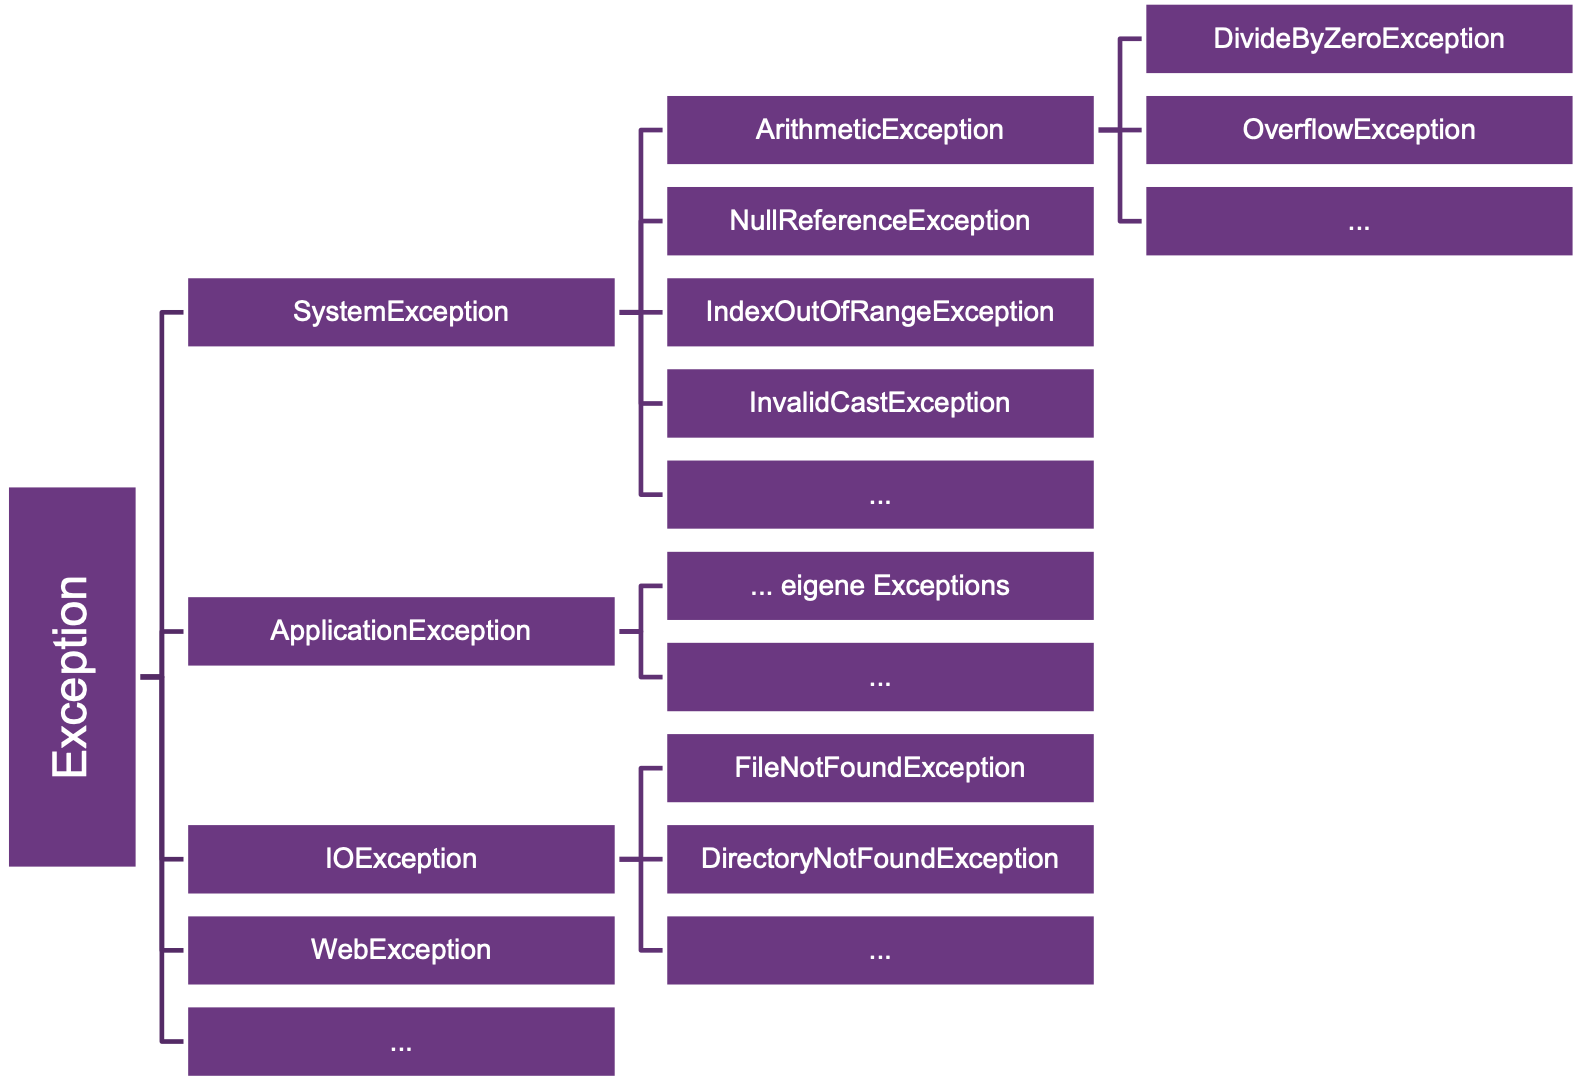
\includegraphics[scale=.25]{graphic/exceptions/Exception-Typen.png}
\end{center}
\vspace{-8pt}

\subsection{Suche nach catch-Klausel}
\begin{itemize}
    \item Call Stack wird rückwärts nach passender «catch» Klausel durchsucht
    \item Programmabbruch mit Fehlermeldung und Stack-Trace falls nicht gefunden
\end{itemize}
\vspace{-8pt}
\begin{center}
    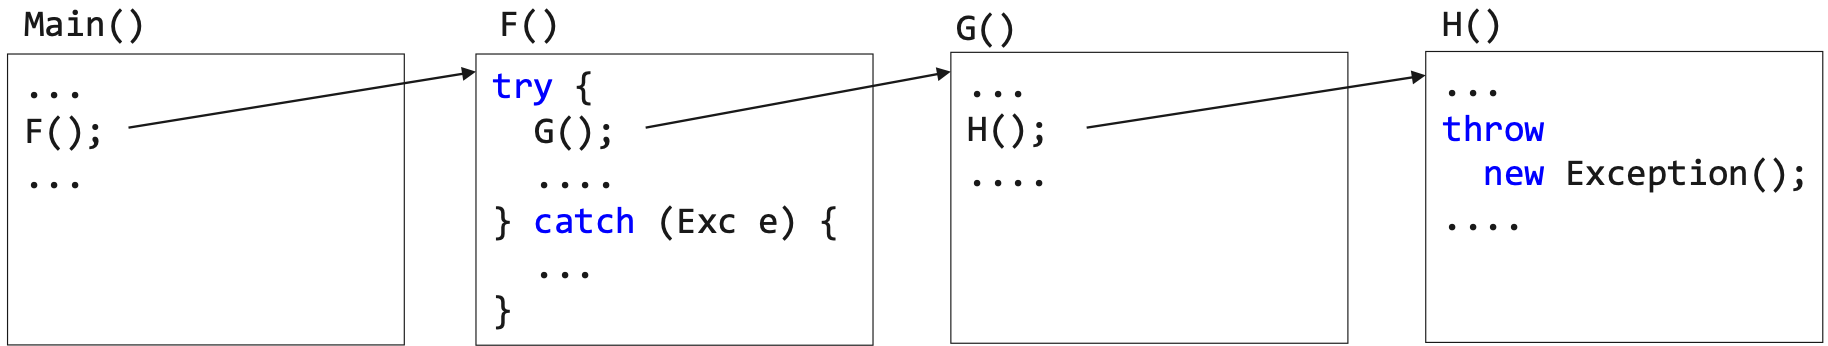
\includegraphics[scale=.25]{graphic/exceptions/Suche.png}
\end{center}
\vspace{-8pt}

\subsubsection{mit Delegates}
\begin{itemize}
    \item Delegates werden wie normale Methoden behandelt
\end{itemize}
\vspace{-8pt}
\begin{center}
    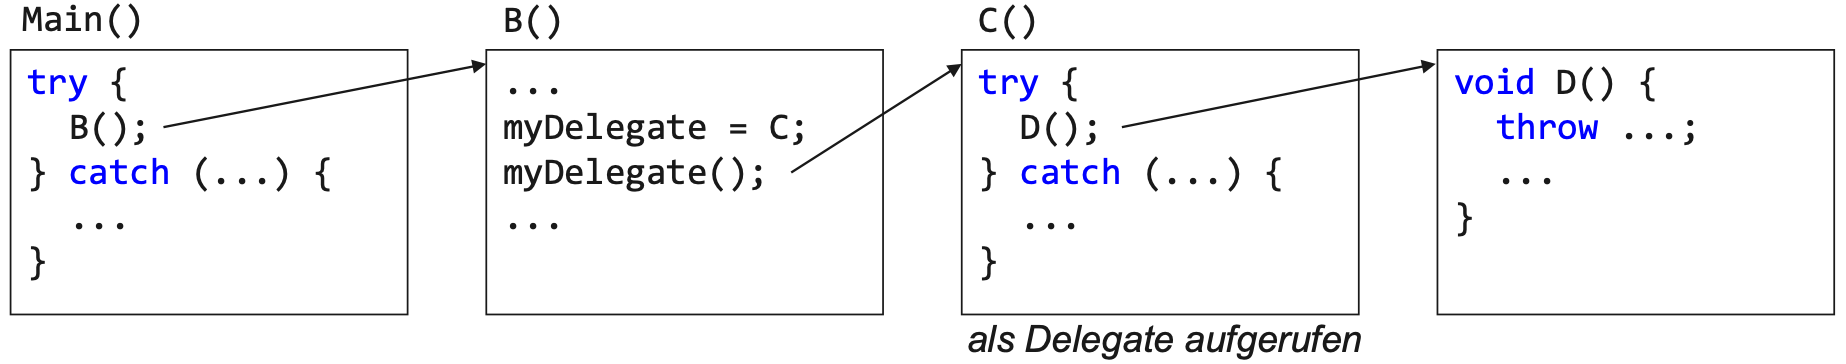
\includegraphics[scale=.25]{graphic/exceptions/suche delegate.png}
\end{center}
\vspace{-8pt}

\subsubsection{mit Multicast-Delegates}
\begin{itemize}
    \item Szenario 1
    \begin{itemize}
        \item Exc1 in G() wird ausgelöst
        \item «catch» für Exc1 in F1() behandelt Ausnahme
        \item F2() wird aufgerufen
    \end{itemize}
    \item Szenario 2
    \begin{itemize}
        \item Exc2 in G() wird ausgelöst
        \item Keine «catch» Klausel für Exc2 gefunden
        \item F2() wird nicht aufgerufen
        \item «catch» für Exc2 in Main() behandelt Ausnahme
    \end{itemize}
\end{itemize}
\vspace{-8pt}
\begin{center}
    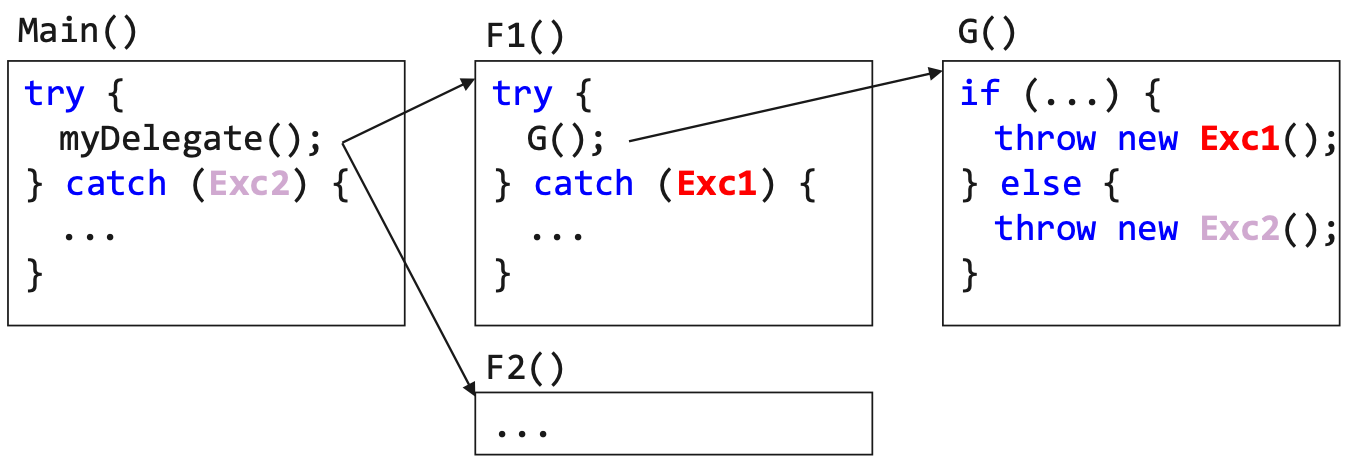
\includegraphics[scale=.27]{graphic/exceptions/suche delegate multicast.png}
\end{center}
\vspace{-8pt}

\subsection{Exception Filters}
Catch-Block wird nur unter definierter Bediungung ausgeführt

\begin{itemize}
    \item «when» Klausel (Zugriff auf Exception möglich)
    \item Erwartet «bool» Expression
\end{itemize}
\begin{lstlisting}
try {
    /* ... */
}
catch (Exception e) when (DateTime.Now.Hour < 18) {
    /* ... */
}
catch (Exception e) when (DateTime.Now.Hour >= 18) {
    /* ... */}
\end{lstlisting}

\subsection{Unchecked Exceptions}
Aufrufer von myMethod() können Exception
behandeln, müssen aber nicht.
\begin{itemize}
    \item Kürzer und bequemer 
    \item Weniger sicher und robust 
\end{itemize}
\begin{lstlisting}
void myMethod() {
    throw new IOException(); }
\end{lstlisting}

\subsection{Argumente prüfen}
Zwei verschiedene Ausprägungen:
\begin{itemize}
    \item ArgumentNullException
    \begin{itemize}
        \item bei null-Werten
    \end{itemize}
    \item ArgumentOutOfRangeException
    \begin{itemize}
        \item bei ungültigen Wertebereichen
    \end{itemize}
\end{itemize}

\hrule

Verwendung des «nameof» Operators:
\begin{itemize}
    \item Zur Ermittlung des ungültigen Parameter
    \item Refactoring-stabil
\end{itemize}

\begin{lstlisting}
string Replicate(string s, int nTimes) {
    if (s == null) {
        throw new ArgumentNullException(nameof(s));
    }
    if (s.Length == 0) {
        throw new ArgumentOutOfRangeException(nameof(s));
    }
    if (nTimes <= 1) {
        throw new ArgumentOutOfRangeException(nameof(nTimes));
    }
 return new StringBuilder().Insert(0, s, nTimes) .ToString();}
\end{lstlisting}

\newpage